\chapter[Processo de Integração]{\textbf{P}rocesso de \textbf{I}ntegração}
\addcontentsline{toc}{chapter}{Processo de Integração}

\textit{Neste capítulo são apresentados os procedimentos para a integração dos sistemas envolvidos, expondo o detalhes de implementação e configuração da solução proposta.}


\section{Definição da Solução}

Após o estudo aprofundado sobre o sistema GSAN e software Asterisk foram identificadas diversas formas de realizar a integração, entre os sistemas pelo fato da existência de várias protocolos possíveis de comunicação , no entanto a solução adotada será visando a reusabilidade, baixo custo de manutenção e o uso de tecnologias que já tenham uma maturidade no mercado. Foram escolhidos os protocolos SOAP e AGI para serem implementados por um \textit{Middleware}, este será responsável em assumir o papel de intermediário entre os sistemas GSAN e Asteisk. Com o intuito de facilitar o entendimento da comunicação entre os sistemas, a seguir será exposto o diagrama de implantação da solução (figura 9) descrita acima, explanado os principais detalhes adotados nesta integração:

% 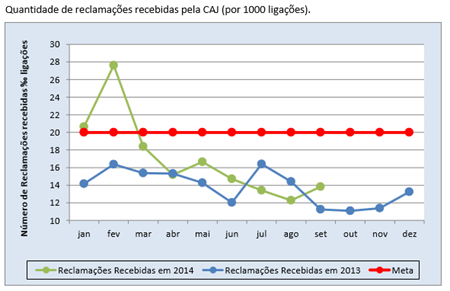
\includegraphics{figuras/LigacoesReclamacoes}
\begin{center}
	IMAGEM PENDENTE \\
	Figura 9: Diagrama de implantação da solução \\
	Fonte: Autoria Própria	\\
\end{center}

Conforme ilustrado acima, o sistema GSAN irá prover uma interface de serviços na forma de WebServices utilizando o protocolo de comunicação SOAP (\textit{Simple Object Access Protocol}), tais serviços serão consumidos através do \textit{Middleware} intermediário denominado integrador que além de consumir os serviços do sistema GSAN, deverá também prover uma interface de serviços na forma utilizando o protocolo AGI, para então ser consumidos pelo Asterisk e responder a solicitação da Unidade de Resposta Audível.


\section{Tecnologias Utilizadas}
O processo de integração será composto por tecnologias com paradigmas diferenciados, no entanto para melhorar o entendimento dos detalhes de compatibilidades adotados segue abaixo a tabela 3 das tecnologias utilizadas e versões correspondentes.

TABELA